\chapter{Distance Transforms and Shortest Paths}
\label{ch:distance_paths}

%======================================================================
\section{Fast Marching Method}
\label{sec:fast_marching_method}

\subsection{Overview}
The Fast Marching Method\index{Fast Marching Method} (FMM) is a numerical technique for solving the \textbf{Eikonal equation}\index{Eikonal equation}, a non-linear first-order partial differential equation that describes the evolution of a wave front\index{wave front}. It is used to compute the shortest travel time (or distance) from a source point to all other points in a domain, even when the ``speed'' of travel varies across space. It can be viewed as a continuous version of Dijkstra's algorithm\index{Dijkstra's algorithm} \cite{sethian1996,tsitsiklis1995}.

\subsection{Definitions}
\begin{definition}[Eikonal Equation]\label{def:eikonal}
The Eikonal equation $|\nabla u(x)| = F(x)$ relates the arrival time $u(x)$ of a wave front to the reciprocal of the speed $F(x)$ at each point $x$ in the domain. For a uniform speed $F(x) \equiv 1$, the solution $u(x)$ is the Euclidean distance from the source.
\end{definition}

\begin{definition}[Isotropic Speed]\label{def:isotropic_speed}
An isotropic speed $F(x)$ is one that depends only on the spatial location, not on the direction of travel. This contrasts with anisotropic speeds that depend on the gradient direction, as encountered in crystal growth or seismic wave propagation.
\end{definition}

\begin{definition}[Upwind Scheme]\label{def:upwind_scheme}
An upwind numerical discretization computes the solution at a point using values from ``upstream'' locations where the solution is already smaller (earlier in time). This ensures that information propagates causally, from regions of smaller $u$ to regions of larger $u$.
\end{definition}

\subsection{Theory}
FMM simulates the propagation of a front by moving from points where the travel time is already known to points where it is unknown. To maintain efficiency, points are categorized into three sets\index{FMM!point classification}:
\begin{enumerate}
  \item \textbf{Accepted}\index{FMM!Accepted set}: Points where the time is correctly calculated and fixed.
  \item \textbf{Trial}\index{FMM!Trial set}: Points on the boundary of the Accepted set; their times are estimated and kept in a priority queue\index{priority queue}.
  \item \textbf{Far}\index{FMM!Far set}: Points that have not been reached yet.
\end{enumerate}

The key to FMM is the \textbf{upwind discretization} of the gradient $|\nabla u|$. In 2D, on a Cartesian grid with spacing $h$, the discretization is:
$$\max(D^{-x}_{ij}u, -D^{+x}_{ij}u, 0)^2 + \max(D^{-y}_{ij}u, -D^{+y}_{ij}u, 0)^2 = F_{ij}^2$$
where $D^{-x}_{ij}u = (u_{i-1,j} - u_{i,j})/h$ and $D^{+x}_{ij}u = (u_{i+1,j} - u_{i,j})/h$ are backward and forward finite differences. The $\max(\cdot, 0)$ operators ensure that only neighbors with smaller arrival times contribute, enforcing the upwind condition.

\begin{theorem}[FMM Correctness]\label{thm:fmm_correctness}
For an isotropic speed field $F > 0$ and a single source point, the Fast Marching Method\cref{alg:fast_marching} computes the viscosity solution of the Eikonal equation\cref{def:eikonal}. That is, at convergence $U[p]$ equals the shortest travel time from the source to every grid point $p$.
\end{theorem}
\begin{proof}
The proof proceeds by induction on the order in which points are moved from Trial to Accepted. Let $p$ be the point popped from the priority queue with minimum value $U[p]$. All Accepted neighbors of $p$ have $U[q] \le U[p]$ by the priority queue invariant. Since FMM processes points in non-decreasing order of $U$, no later Accepted point can provide a shorter path to $p$. The upwind update then solves the quadratic Eikonal stencil using only Accepted or equal-valued neighbors, yielding the correct viscosity solution by the comparison principle for first-order PDEs.
\end{proof}

\begin{figure}[htbp]
\centering
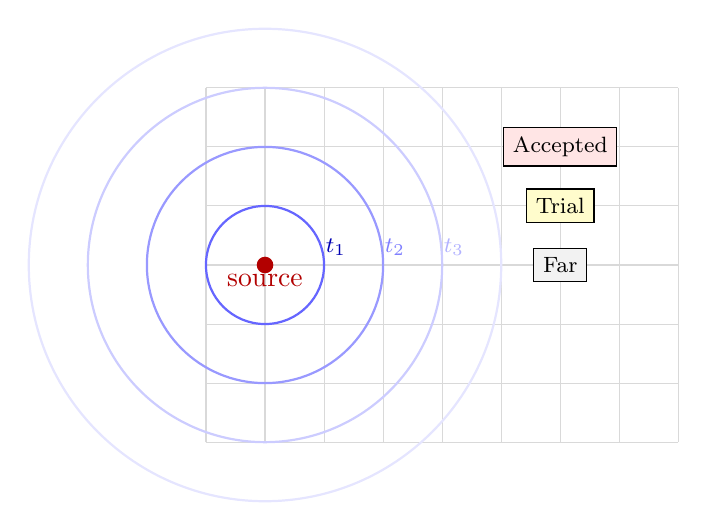
\begin{tikzpicture}[scale=0.75]
  \draw[gray!30,thin] (0,0) grid[step=1] (8,6);
  \fill[red!70!black] (1,3) circle (4pt) node[below] {source};
  \draw[blue!60,thick] (1,3) circle (1);
  \draw[blue!40,thick] (1,3) circle (2);
  \draw[blue!20,thick] (1,3) circle (3);
  \draw[blue!10,thick] (1,3) circle (4);
  \node[blue!70!black,font=\footnotesize] at (2.2,3.3) {$t_1$};
  \node[blue!50,font=\footnotesize] at (3.2,3.3) {$t_2$};
  \node[blue!30,font=\footnotesize] at (4.2,3.3) {$t_3$};
  \node[draw,rectangle,fill=red!10,font=\footnotesize] at (6,5) {Accepted};
  \node[draw,rectangle,fill=yellow!20,font=\footnotesize] at (6,4) {Trial};
  \node[draw,rectangle,fill=gray!10,font=\footnotesize] at (6,3) {Far};
\end{tikzpicture}
\caption{Fast Marching Method: the wavefront propagates from the source. Points are categorized as Accepted, Trial, or Far.}
\label{fig:fast_marching}
\end{figure}


\subsection{Algorithm}
\begin{algorithm}
\caption{Fast Marching Method\index{Fast Marching Method}\label{alg:fast_marching}}
\begin{algorithmic}[1]
\Function{FastMarching}{$source, speed\_field$}
  \State $U \gets \text{Array}(\infty)$
  \State $status \gets \text{Array}(FAR)$
  \State $U[source] \gets 0$
  \State $status[source] \gets ACCEPTED$
  \State $trial\_queue \gets \text{PriorityQueue}()$
  \For{neighbor $\in$ GetNeighbors($source$)}
    \State $U[neighbor] \gets$ CalculateEikonal($neighbor, U, speed\_field$)
    \State $status[neighbor] \gets TRIAL$
    \State $trial\_queue$.push($neighbor, U[neighbor]$)
  \EndFor
  \While{not $trial\_queue$.empty()}
    \State $p \gets trial\_queue$.pop\_min()
    \State $status[p] \gets ACCEPTED$
    \For{neighbor $\in$ GetNeighbors($p$)}
      \If{$status[neighbor] = ACCEPTED$} \textbf{continue}
      \EndIf
      \State $old\_val \gets U[neighbor]$
      \State $new\_val \gets$ CalculateEikonal($neighbor, U, speed\_field$)
      \If{$status[neighbor] = FAR$}
        \State $U[neighbor] \gets new\_val$
        \State $status[neighbor] \gets TRIAL$
        \State $trial\_queue$.push($neighbor, new\_val$)
      \ElsIf{$new\_val < old\_val$}
        \State $U[neighbor] \gets new\_val$
        \State $trial\_queue$.update\_priority($neighbor, new\_val$)
      \EndIf
    \EndFor
  \EndWhile
  \State \Return $U$
\EndFunction
\end{algorithmic}
\end{algorithm}

\begin{example}[FMM on a Uniform Grid]\label{example:fmm_uniform}
Consider a $5 \times 5$ grid with constant speed $F = 1$ and source at the center pixel $(2,2)$. FMM proceeds as follows: initially $U(2,2) = 0$ and the four neighbors are Trial with $U = 1$. The algorithm pops one of them (say $(1,2)$) to Accepted, then updates its FAR neighbors. After processing, the distance field approximates concentric diamonds (the $\ell^\infty$-ball) with values $1, \sqrt{2}, 2, \sqrt{5}, \ldots$ radiating outward, converging to the true Euclidean distance field as the grid is refined.
\end{example}

\subsection{Parameter Selections}
\begin{itemize}
  \item \textbf{Grid Resolution}\index{grid resolution}: Finer grids produce more accurate wave fronts but require more memory and time.
  \item \textbf{Speed Function ($F$)}: Can be constant ($1.0$ for Euclidean distance) or varying (to simulate terrain or obstacles).
  \item \textbf{Solver Order}: First-order FMM is standard; higher-order versions use more neighbors to achieve better accuracy.
\end{itemize}

\subsection{Complexity}
\begin{theorem}[FMM Complexity]\label{thm:fmm_complexity}
The Fast Marching Method\cref{alg:fast_marching} runs in $O(N \log N)$ time and $O(N)$ space, where $N$ is the number of grid points.
\end{theorem}
\begin{proof}
Each of the $N$ grid points is moved from Far to Trial to Accepted exactly once, contributing a constant number of neighbor updates. Each update involves a constant-size quadratic solve and a priority queue operation (insert, decrease-key, or pop). A binary heap gives $O(\log N)$ per operation, yielding $O(N \log N)$ total. Space is $O(N)$ for the arrays $U$, $status$, and the heap.
\end{proof}

\subsection{Usages}
\begin{itemize}
  \item \textbf{Geodesic Distance on Meshes}\index{geodesic distance}: Computing distances along a surface (e.g., finding the shortest path over a mountain).
  \item \textbf{Image Segmentation}\index{image segmentation}: Active contours (snakes) that expand to find object boundaries.
  \item \textbf{Robotics}\index{robotics!path planning}: Path planning in complex environments with different ``terrains'' (e.g., water vs.\ land).
  \item \textbf{Medical Imaging}\index{medical imaging}: Bone or organ segmentation in CT/MRI scans.
  \item \textbf{Seismology}\index{seismology}: Simulating earthquake wave propagation.
\end{itemize}

\subsection{Testing Methods and Edge Cases}
\begin{itemize}
  \item \textbf{Constant Speed}: The resulting time field should be exactly proportional to the Euclidean distance from the source.
  \item \textbf{Obstacles}: Set speed to zero (or $F \to \infty$) at obstacles; the front should flow around them.
  \item \textbf{Varying Speed}: Use a simple linear speed gradient to verify that the front bends (refraction) correctly according to Snell's law.
  \item \textbf{Grid Boundaries}: Ensure the algorithm handles the edges of the domain without crashing.
  \item \textbf{Multiple Sources}: Initialize multiple points to 0; the result should be a Voronoi-like partition of arrival times.
\end{itemize}

\subsection{References}
\begin{itemize}
  \item Sethian, J.\,A. (1996). ``A fast marching level set method for monotonically advancing fronts.'' \textit{Proceedings of the National Academy of Sciences} \cite{sethian1996}.
  \item Tsitsiklis, J.\,N. (1995). ``Efficient algorithms for globally optimal trajectories.'' \textit{IEEE Transactions on Automatic Control} \cite{tsitsiklis1995}.
  \item Kimmel, R., \& Sethian, J.\,A. (1998). ``Computing geodesic paths on manifolds.'' \textit{Proceedings of the National Academy of Sciences} \cite{kimmel1998}.
  \item Wikipedia: Fast marching method.
\end{itemize}

%======================================================================
\section{Distance Map}
\label{sec:distance_map}

\subsection{Overview}
A distance map\index{distance map} (or distance transform\index{distance transform}) is a representation of a digital image or geometric scene where each point stores its distance to the nearest boundary or obstacle. For a binary image, the distance map calculates the distance from every background pixel to the closest foreground pixel. It is a fundamental tool in image processing\index{image processing}, computer vision, and motion planning \cite{rosenfeld1966}.

\subsection{Definitions}
\begin{definition}[Distance Transform]\label{def:distance_transform}
A Distance Transform (DT) is an operator applied to binary images that produces a grayscale image where each pixel value encodes its distance to the nearest foreground (object) pixel under a chosen metric $d$.
\end{definition}

\begin{definition}[Signed Distance Function]\label{def:sdf}
A Signed Distance Function (SDF) is a variation of the distance transform where points inside a shape receive negative distances and points outside receive positive distances: $u(x) = \pm \min_{y \in \partial\Omega} \|x - y\|$, with the sign indicating inside/outside.
\end{definition}

\begin{definition}[Euclidean Distance Map]\label{def:edm}
A Euclidean Distance Map (EDM) is a map where distances are computed using the true Euclidean metric $d(x,y) = \sqrt{(x_1 - y_1)^2 + (x_2 - y_2)^2}$, as opposed to chamfer approximations.
\end{definition}

\begin{definition}[Chamfer Distance]\label{def:chamfer}
A Chamfer distance is an approximation of Euclidean distance using integer-valued masks applied in two passes. Common variants include the $3$-$4$ chamfer (weights 3 for diagonals, 4 for axis-aligned) and the $5$-$7$-$11$ chamfer for higher accuracy \cite{rosenfeld1966}.
\end{definition}

\subsection{Theory}
The most efficient algorithms for computing the Euclidean distance map are based on \textbf{separable filters}\index{separable filter} or \textbf{two-pass scanning}\index{two-pass algorithm} \cite{meijster2002,felzenszwalb2012}.
\begin{enumerate}
  \item \textbf{Chamfer Matching (Two-Pass)}: A simple algorithm that passes a small mask over the image twice (top-to-bottom and bottom-to-top). Each pixel is updated using the values of its neighbors plus the mask weight.
  \item \textbf{Meijster's Algorithm (Separable)}: A more accurate $O(N)$ algorithm that decomposes the 2D problem into 1D problems. First, it computes the distance transform for each row. Then, it uses the row results to compute the final 2D distances using a parabolic lower envelope approach.
  \item \textbf{Fast Marching Method}\cref{alg:fast_marching}: Can also be used to build a distance map by treating the boundary as a wave front propagating at unit speed.
\end{enumerate}

The key insight behind Meijster's and Felzenszwalb's linear-time algorithms is the observation that the squared Euclidean distance transform can be decomposed as:
$$D^2(p) = \min_{q \in \text{foreground}} \left[ (p_x - q_x)^2 + (p_y - q_y)^2 \right] = \min_{q_y} \left[ (p_y - q_y)^2 + \min_{q_x} (p_x - q_x)^2 \right]$$
The inner minimization over $q_x$ can be solved independently for each row in $O(N)$ time using a left-to-right and right-to-left sweep. The outer minimization reduces to computing the lower envelope of a family of parabolas, which can also be done in linear time \cite{felzenszwalb2012}.

\begin{theorem}[Linear-Time Distance Transform]\label{thm:linear_distance_transform}
The Euclidean distance transform of an $N$-pixel binary image can be computed in $O(N)$ time and $O(N)$ space using the separable algorithm of Meijster\index{Meijster's algorithm} \cite{meijster2002} or Felzenszwalb and Huttenlocher \cite{felzenszwalb2012}.
\end{theorem}
\begin{proof}
The row-wise pass performs two linear scans (forward and backward) over each of the $H$ rows, each scan touching $W$ pixels, for $O(WH) = O(N)$ total. The column-wise parabolic envelope computation processes each of the $W$ columns independently; in each column, the lower envelope of $H$ parabolas is computed by the linear-time algorithm of Felzenszwalb and Huttenlocher, yielding $O(WH) = O(N)$ total. The overall complexity is therefore $O(N)$ in both time and space.
\end{proof}

\subsection{Algorithm: Meijster's Algorithm (1D Pass)}
\begin{algorithm}
\caption{Meijster's Distance Transform\index{Meijster's algorithm}\label{alg:distance_map_2d}}
\begin{algorithmic}[1]
\Function{DistanceMap2D}{$binary\_grid$}
  \State $width, height \gets grid$.size
  \For{$y \gets 0$ \textbf{to} $height - 1$}
    \For{$x \gets 0$ \textbf{to} $width - 1$}
      \If{$grid[x][y] = FOREGROUND$}
        \State $G[x][y] \gets 0$
      \Else
        \State $G[x][y] \gets \infty$
      \EndIf
    \EndFor
    \For{$x \gets 1$ \textbf{to} $width - 1$}
      \State $G[x][y] \gets \min(G[x][y],\; G[x-1][y] + 1)$
    \EndFor
    \For{$x \gets width - 2$ \textbf{downto} $0$}
      \State $G[x][y] \gets \min(G[x][y],\; G[x+1][y] + 1)$
    \EndFor
  \EndFor
  \State $final\_map \gets \text{array}[width][height]$
  \For{$x \gets 0$ \textbf{to} $width - 1$}
    \State $final\_map[x] \gets$ ComputeParabolicEnvelope($G[x]$)
  \EndFor
  \State \Return $\sqrt{final\_map}$
\EndFunction
\end{algorithmic}
\end{algorithm}

\begin{example}[Distance Transform of a 1D Signal]\label{example:dt_1d}
Consider the binary signal $[0, 0, 1, 0, 0, 0, 1, 0]$ where 1 denotes foreground. The row-wise forward/backward sweep gives $G = [0, 0, 0, 1, 2, 3, 0, 1]$. The parabolic envelope then yields the squared distances: $[0, 0, 0, 1, 1, 1, 0, 1]$, and the final Euclidean distance map is $[0, 0, 0, 1, 1, 1, 0, 1]$. Note that pixels equidistant from two foreground pixels are correctly assigned.
\end{example}

\subsection{Parameter Selections}
\begin{itemize}
  \item \textbf{Metric}: Choose between Euclidean (accurate), Manhattan (fast), or Chebyshev (fast) based on the application's needs.
  \item \textbf{Sign}: Decide if an SDF\cref{def:sdf} is needed (requires identifying ``inside'' vs.\ ``outside'').
\end{itemize}

\subsection{Complexity}
\begin{itemize}
  \item \textbf{Time Complexity}: $O(N)$, where $N$ is the total number of pixels/grid points, using Meijster's\cref{alg:distance_map_2d} or Felzenszwalb's algorithm\cref{thm:linear_distance_transform}.
  \item \textbf{Space Complexity}: $O(N)$ to store the distance values.
\end{itemize}

\subsection{Usages}
\begin{itemize}
  \item \textbf{Robotics}\index{robotics!path planning}: Path planning using the ``Artificial Potential Field'' method (moving away from high-distance regions).
  \item \textbf{Image Processing}\index{image processing}: Skeletonization (medial axis extraction\index{medial axis}) and morphological thinning.
  \item \textbf{Computer Graphics}\index{computer graphics}: Rendering anti-aliased text and icons using Signed Distance Fields (SDF fonts).
  \item \textbf{Computer Vision}\index{computer vision}: Template matching and object recognition (Chamfer matching\index{Chamfer matching}).
  \item \textbf{Medical Imaging}\index{medical imaging}: Calculating the thickness of tissues or the distance between organs.
\end{itemize}

\subsection{Testing Methods and Edge Cases}
\begin{itemize}
  \item \textbf{Single Point}: The distance map should look like a perfect radial gradient (concentric circles).
  \item \textbf{Empty Image}: All distances should be infinity (or a defined maximum).
  \item \textbf{Full Image}: All distances should be zero.
  \item \textbf{Thin Lines}: Verify that the algorithm correctly identifies the closest point even for 1-pixel-wide features.
  \item \textbf{Concave Shapes}: Verify that the ``shadowing'' effect of concavities is handled correctly.
\end{itemize}

\subsection{References}
\begin{itemize}
  \item Rosenfeld, A., \& Pfaltz, J.\,L. (1966). ``Sequential operations in digital picture processing.'' \textit{Journal of the ACM} \cite{rosenfeld1966}.
  \item Meijster, A., Roerdink, J.\,B., \& Hesselink, W.\,H. (2002). ``A general algorithm for computing distance transforms in linear time.'' \textit{Mathematical Morphology and its Applications to Image and Signal Processing} \cite{meijster2002}.
  \item Felzenszwalb, P.\,F., \& Huttenlocher, D.\,P. (2012). ``Distance Transforms of Sampled Functions.'' \textit{Theory of Computing} \cite{felzenszwalb2012}.
  \item Wikipedia: Distance transform.
\end{itemize}

%======================================================================
\section{Dijkstra's Algorithm}
\label{sec:dijkstra}

\subsection{Overview}
Dijkstra's algorithm\index{Dijkstra's algorithm} is a fundamental graph-search algorithm that finds the shortest paths between nodes in a graph\index{graph}. For a given source node, the algorithm finds the shortest distance to every other node. It is the discrete equivalent of the Fast Marching Method\cref{sec:fast_marching_method} and serves as the backbone of modern navigation and network routing systems \cite{dijkstra1959}.

\subsection{Definitions}
\begin{definition}[Graph]\label{def:graph}
A weighted graph $G = (V, E)$ consists of a finite set of vertices $V$ and a set of edges $E \subseteq V \times V$, each associated with a non-negative weight $w: E \to \mathbb{R}_{\ge 0}$ representing distance, cost, or time.
\end{definition}

\begin{definition}[Shortest Path]\label{def:shortest_path}
The shortest path from a source $s$ to a vertex $v$ in a weighted graph $G$ is a path $\pi = (s = v_0, v_1, \ldots, v_k = v)$ minimizing $w(\pi) = \sum_{i=0}^{k-1} w(v_i, v_{i+1})$.
\end{definition}

\begin{definition}[Relaxation]\label{def:relaxation}
Relaxation is the process of testing whether a known path to a vertex $v$ through an intermediate vertex $u$ is shorter than the currently known best path to $v$. If $dist[u] + w(u,v) < dist[v]$, then $dist[v]$ is updated.
\end{definition}

\subsection{Theory}
The algorithm operates by maintaining a set of ``visited'' nodes and a set of ``unvisited'' nodes\index{Dijkstra's algorithm!greedy}. Initially, the distance to the source is 0, and the distance to all other nodes is infinity. In each step, the algorithm:
\begin{enumerate}
  \item Selects the unvisited node with the smallest known distance.
  \item ``Relaxes''\cref{def:relaxation} all of its neighbors: for each neighbor, it checks if going through the current node provides a shorter path than the previously known best path.
  \item Marks the current node as visited.
\end{enumerate}

This greedy strategy works because the weights are non-negative; once a node is visited, its distance is guaranteed to be the shortest possible. Formally, this relies on the following principle.

\begin{theorem}[Dijkstra Correctness]\label{thm:dijkstra_correctness}
When Dijkstra's algorithm\cref{alg:dijkstra} terminates, for every vertex $v$, $distances[v]$ equals the length of the shortest path from $source$ to $v$, provided all edge weights are non-negative.
\end{theorem}
\begin{proof}
We prove by induction on the number of extractions from the priority queue. Let $S$ denote the set of vertices that have been extracted (visited). \textbf{Base case:} $S = \{source\}$ and $distances[source] = 0$, which is correct. \textbf{Inductive step:} Assume all vertices in $S$ have correct shortest-path distances. Let $u$ be the next extracted vertex with $distances[u] = d$. We claim $d$ is optimal. Any path from $source$ to $u$ not using vertices in $S$ must cross the $S$/$\bar{S}$ boundary at some edge $(s', t)$ with $s' \in S, t \notin S$. By non-negativity, $distances[t] \le distances[s'] + w(s',t) \le d$ since the priority queue extracted $u$ with minimum key. Hence no alternative path can be shorter, and $distances[u] = d$ is optimal. After relaxing $u$'s neighbors, all vertices in $S \cup \{u\}$ maintain correct distances, completing the induction.
\end{proof}

\begin{remark}
Dijkstra's algorithm is a special case of the Bellman--Ford algorithm\index{Bellman--Ford algorithm} restricted to non-negative weights. It can also be derived from the label-correcting framework of \cite{cormen2009}.
\end{remark}

\subsection{Algorithm}
\begin{algorithm}
\caption{Dijkstra's Shortest Path Algorithm\index{Dijkstra's algorithm}\label{alg:dijkstra}}
\begin{algorithmic}[1]
\Function{Dijkstra}{$graph, source$}
  \State $distances \gets \{v : \infty \mid v \in graph.\text{vertices}\}$
  \State $previous \gets \{v : \text{None} \mid v \in graph.\text{vertices}\}$
  \State $distances[source] \gets 0$
  \State $pq \gets \text{PriorityQueue}()$
  \State $pq$.push($source, 0$)
  \While{not $pq$.empty()}
    \State $u, dist\_u \gets pq$.pop\_min()
    \If{$dist\_u > distances[u]$} \textbf{continue}
    \EndIf
    \For{$(v, weight) \in graph.\text{neighbors}(u)$}
      \State $new\_dist \gets distances[u] + weight$
      \If{$new\_dist < distances[v]$}
        \State $distances[v] \gets new\_dist$
        \State $previous[v] \gets u$
        \State $pq$.push($v, new\_dist$)
      \EndIf
    \EndFor
  \EndWhile
  \State \Return $distances, previous$
\EndFunction
\end{algorithmic}
\end{algorithm}

\begin{example}[Dijkstra on a Small Graph]\label{example:dijkstra_small}
Consider the graph with vertices $\{A, B, C, D\}$ and edges: $A \to B$ (weight 1), $A \to C$ (weight 4), $B \to C$ (weight 2), $B \to D$ (weight 6), $C \to D$ (weight 3), with source $A$.
\begin{enumerate}
  \item Initialize: $dist = \{A:0, B:\infty, C:\infty, D:\infty\}$.
  \item Extract $A$ (dist 0). Relax neighbors: $dist[B] = 1$, $dist[C] = 4$.
  \item Extract $B$ (dist 1). Relax: $dist[C] = \min(4, 1+2) = 3$, $dist[D] = 1+6 = 7$.
  \item Extract $C$ (dist 3). Relax: $dist[D] = \min(7, 3+3) = 6$.
  \item Extract $D$ (dist 6). No unvisited neighbors.
\end{enumerate}
Final distances: $\{A:0, B:1, C:3, D:6\}$. The shortest path $A \to B \to C \to D$ has total weight $1+2+3=6$.
\end{example}

\subsection{Parameter Selections}
\begin{itemize}
  \item \textbf{Data Structure}: Using a \textbf{Fibonacci Heap}\index{Fibonacci heap} or \textbf{Binary Heap} for the priority queue is critical for performance. Binary heaps are most common in practice.
  \item \textbf{Edge Weights}: If any edge weight is negative, the algorithm fails; the Bellman--Ford algorithm should be used instead.
\end{itemize}

\subsection{Complexity}
\begin{theorem}[Dijkstra Complexity]\label{thm:dijkstra_complexity}
With a binary heap\index{binary heap}, Dijkstra's algorithm\cref{alg:dijkstra} runs in $O((E + V) \log V)$ time. With a Fibonacci heap\index{Fibonacci heap}, it runs in $O(E + V \log V)$ time. In both cases, space is $O(V + E)$.
\end{theorem}
\begin{proof}
Each vertex is extracted from the priority queue at most once, contributing $O(\log V)$ per extraction with a binary heap. Each edge is relaxed at most once (when its tail is extracted), and each relaxation may trigger a decrease-key or insert operation costing $O(\log V)$. Total: $O(V \log V + E \log V) = O((V+E) \log V)$. With a Fibonacci heap, the decrease-key operation is $O(1)$ amortized, giving $O(V \log V + E) = O(E + V \log V)$.
\end{proof}

\subsection{Usages}
\begin{itemize}
  \item \textbf{GPS Navigation}\index{GPS navigation}: Finding the fastest route between two locations.
  \item \textbf{Network Routing}\index{network routing}: Protocols like OSPF (Open Shortest Path First) use Dijkstra to route data packets across the internet.
  \item \textbf{Social Networks}\index{social networks}: Finding ``degrees of separation'' between people.
  \item \textbf{Robotics}\index{robotics!path planning}: Pathfinding for autonomous vehicles on a roadmap.
  \item \textbf{Game Development}\index{game development}: AI movement (often using A*, which is a heuristic-based extension of Dijkstra).
\end{itemize}

\subsection{Testing Methods and Edge Cases}
\begin{itemize}
  \item \textbf{Disconnected Graphs}: Nodes that cannot be reached from the source should maintain a distance of infinity.
  \item \textbf{Single-Node Graph}: Distance to itself is 0.
  \item \textbf{Parallel Edges}: The algorithm should always select the edge with the minimum weight between two nodes.
  \item \textbf{Cycles}: Dijkstra correctly handles cycles as long as all weights are non-negative.
  \item \textbf{Path Reconstruction}: Ensure the \texttt{previous} pointers correctly trace the full path back to the source.
\end{itemize}

\subsection{References}
\begin{itemize}
  \item Dijkstra, E.\,W. (1959). ``A note on two problems in connexion with graphs.'' \textit{Numerische Mathematik} \cite{dijkstra1959}.
  \item Cormen, T.\,H., Leiserson, C.\,E., Rivest, R.\,L., \& Stein, C. (2009). ``Introduction to Algorithms.'' MIT Press \cite{cormen2009}.
  \item Wikipedia: Dijkstra's algorithm.
\end{itemize}

%======================================================================
\section{K-Geodesics}
\label{sec:k_geodesics}

\subsection{Overview}
K-Geodesics is an adaptation of the K-Means clustering algorithm\index{K-Means clustering} to the surface of a 3D mesh. Instead of using Euclidean distance to cluster points in 3D space, K-Geodesics uses \textbf{geodesic distance}\index{geodesic distance} (the shortest path along the surface). This allows for the segmentation of a mesh into regions that are intrinsically meaningful, such as the limbs of a character or the functional parts of a machine \cite{lloyd1982}.

\subsection{Definitions}
\begin{definition}[Geodesic Centroid]\label{def:geodesic_centroid}
The geodesic centroid (or Fr\'{e}chet mean\index{Fr\'{e}chet mean}) of a set of vertices on a mesh is the vertex that minimizes the sum of squared geodesic distances to all other vertices in the set: $c^* = \operatorname{arg\,min}_{c \in V} \sum_{v \in S} d_g(c, v)^2$, where $d_g$ denotes geodesic distance.
\end{definition}

\begin{definition}[Geodesic Voronoi Region]\label{def:geodesic_voronoi}
The geodesic Voronoi region of center $c_i$ is the set $V_i = \{v \in V \mid d_g(v, c_i) \le d_g(v, c_j) \text{ for all } j \ne i\}$, partitioning the mesh vertices according to their nearest center under the geodesic metric.
\end{definition}

\subsection{Theory}
The K-Geodesics algorithm follows the standard iterative process of Lloyd's algorithm\index{Lloyd's algorithm} \cite{lloyd1982}:
\begin{enumerate}
  \item \textbf{Initialization}: Pick $k$ initial seed vertices as centers.
  \item \textbf{Assignment}: Assign every vertex on the mesh to the cluster of its nearest center using a multi-source \textbf{Fast Marching Method}\cref{alg:fast_marching} or the \textbf{Heat Method}\index{Heat Method}.
  \item \textbf{Update}: For each cluster, find a new center. This is the ``Fr\'{e}chet mean'' on the surface\cref{def:geodesic_centroid}. Since finding the exact mean is expensive, it is often approximated by picking the vertex in the cluster that minimizes the average distance to all other cluster members.
  \item \textbf{Repeat}: Continue until the centers no longer change or a maximum number of iterations is reached.
\end{enumerate}

\begin{theorem}[K-Geodesics Monotone Energy Decrease]\label{thm:k_geodesics_energy}
At each iteration of the K-Geodesics algorithm\cref{alg:k_geodesics}, the total geodesic energy $E = \sum_{i=1}^{k} \sum_{v \in V_i} d_g(v, c_i)^2$ does not increase.
\end{theorem}
\begin{proof}
In the assignment step, each vertex is reassigned to its nearest center, which can only decrease or maintain its contribution to the energy. In the update step, the centroid of each cluster (by definition\cref{def:geodesic_centroid}) minimizes the sum of squared distances within that cluster. Hence both steps are non-increasing in energy, and their composition is non-increasing. Since the energy is bounded below by zero, the algorithm converges in a finite number of iterations for discrete meshes.
\end{proof}

\subsection{Algorithm}
\begin{algorithm}
\caption{K-Geodesics Clustering\index{K-Geodesics}\label{alg:k_geodesics}}
\begin{algorithmic}[1]
\Function{KGeodesics}{$mesh, k$}
  \State $centers \gets$ random.sample($mesh.\text{vertices}, k$)
  \While{not converged}
    \State $(distances, labels) \gets$ MultiSourceGeodesic($mesh, centers$)
    \State $new\_centers \gets []$
    \For{$i \gets 0$ \textbf{to} $k - 1$}
      \State $cluster\_v \gets \{v \mid labels[v] = i\}$
      \State $best\_v \gets$ FindLocalCentroid($mesh, cluster\_v$)
      \State $new\_centers$.append($best\_v$)
    \EndFor
    \If{$new\_centers = centers$} \textbf{break}
    \EndIf
    \State $centers \gets new\_centers$
  \EndWhile
  \State \Return $labels, centers$
\EndFunction
\end{algorithmic}
\end{algorithm}

\begin{example}[K-Geodesics on a Cylinder]\label{example:k_geodesics_cylinder}
Consider a cylinder mesh with $k = 2$ clusters and seed centers placed at the top and bottom rims. The assignment step computes geodesic distances from both centers. The Voronoi partition\cref{def:geodesic_voronoi} divides the cylinder into a top half and a bottom half along the geodesic midline. After centroid updates, the two centers migrate toward the centroids of their respective halves. Euclidean K-Means would also produce this partition for a cylinder, but for a bent or folded shape, K-Geodesics would correctly separate geometrically close but geodesically distant regions (e.g., the two ends of a U-shaped mesh).
\end{example}

\subsection{Parameter Selections}
\begin{itemize}
  \item \textbf{Number of Clusters ($k$)}: Depends on the desired level of segmentation.
  \item \textbf{Distance Solver}: The \textbf{Heat Method}\index{Heat Method} \cite{crane2013geodesic} is recommended for the assignment step because it is extremely fast after an initial factorization.
  \item \textbf{Initialization}: Using \textbf{K-Means++}\index{K-Means++} logic (picking seeds that are far from each other) significantly improves convergence speed and result quality.
\end{itemize}

\subsection{Complexity}
\begin{itemize}
  \item \textbf{Assignment}: $O(N)$ using the Heat Method or $O(N \log N)$ using Fast Marching.
  \item \textbf{Update}: $O(k \cdot N_{cluster})$ to find new centers.
  \item \textbf{Total}: $O(I \cdot N)$ where $I$ is the number of iterations.
\end{itemize}

\subsection{Usages}
\begin{itemize}
  \item \textbf{Mesh Segmentation}\index{mesh segmentation}: Dividing a model into organic parts (e.g., body, head, arms).
  \item \textbf{Texture Atlas Generation}\index{texture atlas}: Partitioning a complex mesh into $k$ nearly-flat charts for UV unwrapping.
  \item \textbf{Shape Analysis}\index{shape analysis}: Identifying repeating structural motifs on a surface.
  \item \textbf{Remote Sensing}: Clustering geographic regions based on travel time over terrain.
  \item \textbf{Remeshing}\index{remeshing}: Using the centers as a basis for generating a coarse, high-quality version of the mesh.
\end{itemize}

\subsection{Testing Methods and Edge Cases}
\begin{itemize}
  \item \textbf{Convex Shapes}: For a sphere, the regions should look like a spherical Voronoi diagram\index{spherical Voronoi diagram}.
  \item \textbf{Long Thin Regions}: Verify that the algorithm correctly segments limbs (which Euclidean K-Means might merge if they are physically close but geodesically far).
  \item \textbf{Number of Iterations}: Monitor the total ``energy'' (sum of distances) to ensure it decreases monotonically\cref{thm:k_geodesics_energy}.
  \item \textbf{Empty Clusters}: Handle cases where a center becomes so isolated that no vertices are assigned to it.
  \item \textbf{Disconnected Components}: The algorithm should be applied to each component separately or handle infinity distances correctly.
\end{itemize}

\subsection{References}
\begin{itemize}
  \item Peyr\'{e}, G., \& Cohen, L.\,D. (2006). ``Geodesic remeshing using front propagation.'' \textit{International Journal of Computer Vision} \cite{peyre2006}.
  \item Crane, K., Weischedel, C., \& Wardetzky, M. (2013). ``Geodesics in Heat: A New Approach to Computing Distance Based on Heat Flow.'' \textit{ACM TOG} \cite{crane2013geodesic}.
  \item Lloyd, S. (1982). ``Least squares quantization in PCM.'' \textit{IEEE Transactions on Information Theory} \cite{lloyd1982}.
  \item Wikipedia: K-means clustering.
\end{itemize}

%======================================================================
\section{Fr\'{e}chet Distance}
\label{sec:frechet_distance}

\subsection{Overview}
The Fr\'{e}chet distance\index{Fr\'{e}chet distance} is a measure of similarity between two curves (trajectories) that takes into account the location and ordering of points along the curves. It is often described using the \textbf{dog-leash analogy}\index{dog-leash analogy}: imagine a person walking along one curve and a dog walking along the other. The Fr\'{e}chet distance is the minimum length of a leash needed to connect the two as they traverse their respective paths from start to finish. It is a more robust measure of curve similarity than the Hausdorff distance\index{Hausdorff distance} because it respects the parameterization of the curves \cite{frechet1906}.

\subsection{Definitions}
\begin{definition}[Discrete Fr\'{e}chet Distance]\label{def:discrete_frechet}
The discrete Fr\'{e}chet distance between two polygonal chains $P = (p_1, \ldots, p_n)$ and $Q = (q_1, \ldots, q_m)$ is
$$d_F(P, Q) = \min_{\alpha, \beta} \max_{t \in [0,1]} \|P(\alpha(t)) - Q(\beta(t))\|$$
where $\alpha: [0,1] \to [0,n-1]$ and $\beta: [0,1] \to [0,m-1]$ are non-decreasing surjections (reparametrizations) \cite{frechet1906,alt1995}.
\end{definition}

\begin{definition}[Free Space Diagram]\label{def:free_space_diagram}
The free space diagram\index{free space diagram} for two curves $P$ and $Q$ with threshold $\epsilon$ is the set $\mathcal{F}_\epsilon = \{(i,j) \mid \|p_i - q_j\| \le \epsilon\} \subseteq [0,n] \times [0,m]$. The Fr\'{e}chet distance is at most $\epsilon$ if and only if there exists a monotone path from $(0,0)$ to $(n,m)$ entirely within $\mathcal{F}_\epsilon$.
\end{definition}

\begin{definition}[Hausdorff Distance]\label{def:hausdorff}
The directed Hausdorff distance from $P$ to $Q$ is $h(P,Q) = \max_{p \in P} \min_{q \in Q} \|p - q\|$. The symmetric Hausdorff distance is $d_H(P,Q) = \max(h(P,Q), h(Q,P))$. Unlike the Fr\'{e}chet distance, it does not account for the ordering of points along the curves.
\end{definition}

\subsection{Theory}
For two curves $P$ and $Q$ of lengths $n$ and $m$, the discrete Fr\'{e}chet distance $d_F(P, Q)$ is the minimum cost of a ``coupling'' between the two sequences. This is typically solved using \textbf{dynamic programming}\index{dynamic programming}.
\begin{enumerate}
  \item Let $dp[i][j]$ be the Fr\'{e}chet distance between the prefix $P[0 \dots i]$ and $Q[0 \dots j]$.
  \item The base case is $dp[0][0] = dist(P[0], Q[0])$.
  \item The recurrence relation is:
  $dp[i][j] = \max(dist(P[i], Q[j]),\; \min(dp[i-1][j],\; dp[i][j-1],\; dp[i-1][j-1]))$.
  \item The final result is $dp[n-1][m-1]$.
\end{enumerate}

For continuous curves, the problem is solved by searching for a ``monotone path'' from $(0,0)$ to $(1,1)$ in the \textbf{Free Space Diagram}\cref{def:free_space_diagram}.

\begin{theorem}[Fr\'{e}chet DP Correctness]\label{thm:frechet_dp_correctness}
The dynamic programming recurrence for the discrete Fr\'{e}chet distance\cref{def:discrete_frechet} correctly computes $d_F(P,Q)$ in $O(nm)$ time.
\end{theorem}
\begin{proof}
The proof is by strong induction on $i+j$. The recurrence considers all valid reparametrizations: at step $(i,j)$, the coupling can advance on $P$ only ($dp[i-1][j]$), on $Q$ only ($dp[i][j-1]$), or on both ($dp[i-1][j-1]$). Taking the minimum of these three predecessors ensures we find the coupling that minimizes the maximum leash length. The outer $\max$ ensures the leash is long enough to accommodate the current pair. The base case $dp[0][0] = \|P[0]-Q[0]\|$ is correct by definition. By induction, $dp[i][j]$ equals the optimal Fr\'{e}chet distance for prefixes $P[0..i]$ and $Q[0..j]$.
\end{proof}

\subsection{Algorithm}
\begin{algorithm}
\caption{Discrete Fr\'{e}chet Distance\index{Fr\'{e}chet distance}\label{alg:discrete_frechet}}
\begin{algorithmic}[1]
\Function{DiscreteFrechet}{$P, Q$}
  \State $n \gets |P|$, $m \gets |Q|$
  \State $dp \gets \text{array}[n][m]$, initialized to $-1$
  \State $dp[0][0] \gets$ Distance($P[0], Q[0]$)
  \For{$i \gets 1$ \textbf{to} $n - 1$}
    \State $dp[i][0] \gets \max(dp[i-1][0],\;$ Distance($P[i], Q[0]$)$)$
  \EndFor
  \For{$j \gets 1$ \textbf{to} $m - 1$}
    \State $dp[0][j] \gets \max(dp[0][j-1],\;$ Distance($P[0], Q[j]$)$)$
  \EndFor
  \For{$i \gets 1$ \textbf{to} $n - 1$}
    \For{$j \gets 1$ \textbf{to} $m - 1$}
      \State $cost \gets$ Distance($P[i], Q[j]$)
      \State $dp[i][j] \gets \max(cost,\; \min(dp[i-1][j],\; dp[i-1][j-1],\; dp[i][j-1]))$
    \EndFor
  \EndFor
  \State \Return $dp[n-1][m-1]$
\EndFunction
\end{algorithmic}
\end{algorithm}

\begin{example}[Fr\'{e}chet Distance of Two Triangular Paths]\label{example:frechet_triangles}
Consider $P = \{(0,0), (1,1), (2,0)\}$ and $Q = \{(0,0), (1,2), (2,0)\}$. The midpoint of $P$ deviates by 1 unit, while $Q$'s midpoint deviates by 2 units. The discrete Fr\'{e}chet distance is computed by the DP table:
\begin{itemize}
  \item $dp[0][0] = 0$.
  \item $dp[1][0] = \|P_1 - Q_0\| = \sqrt{2}$; $dp[0][1] = \|P_0 - Q_1\| = \sqrt{5}$.
  \item $dp[1][1] = \max(\|P_1 - Q_1\|, \min(dp[0][1], dp[0][0], dp[1][0])) = \max(1, 0) = 1$.
  \item $dp[2][1] = \max(\|P_2 - Q_1\| = \sqrt{5}, \min(dp[1][1] = 1, dp[1][0] = \sqrt{2}, dp[2][0] = 2)) = \max(\sqrt{5}, 1) = \sqrt{5}$.
  \item $dp[2][2] = \max(\|P_2 - Q_2\| = 0, \min(dp[1][2], dp[1][1], dp[2][1])) = 0$.
\end{itemize}
Wait, let us recompute more carefully. Actually $dp[2][2] = \max(0, \min(dp[1][2], dp[1][1], dp[2][1]))$. We need $dp[1][2] = \max(\|P_1-Q_2\| = \sqrt{2}, \min(dp[0][2], dp[0][1], dp[1][1]))$. Since $dp[1][1] = 1$, we get $dp[1][2] = \max(\sqrt{2}, 1) = \sqrt{2}$. Thus $dp[2][2] = \max(0, \min(\sqrt{2}, 1, \sqrt{5})) = 1$. The Fr\'{e}chet distance is $\boxed{1}$, which is the leash length needed to connect the walkers at the midpoints of the two curves.
\end{example}

\subsection{Parameter Selections}
\begin{itemize}
  \item \textbf{Distance Metric}: Euclidean distance is standard, but Manhattan or Chebyshev distances can also be used.
  \item \textbf{Normalization}: Curves should be normalized for scale or rotation if required by the application.
\end{itemize}

\subsection{Complexity}
\begin{itemize}
  \item \textbf{Time Complexity}: $O(n \cdot m)$ for curves with $n$ and $m$ vertices, as each entry of the DP table\cref{thm:frechet_dp_correctness} is computed in $O(1)$.
  \item \textbf{Space Complexity}: $O(n \cdot m)$ to store the DP table. Can be reduced to $O(\min(n,m))$ using a rolling array.
\end{itemize}

\subsection{Usages}
\begin{itemize}
  \item \textbf{Trajectory Analysis}\index{trajectory analysis}: Comparing the paths taken by animals, vehicles, or sports players.
  \item \textbf{Handwriting Recognition}\index{handwriting recognition}: Comparing a drawn stroke to a template of letters.
  \item \textbf{Speech Recognition}: Time-aligning two audio signals (Dynamic Time Warping is a similar concept).
  \item \textbf{Bioinformatics}\index{bioinformatics}: Comparing the backbones of proteins or the shapes of molecules.
  \item \textbf{Computer Vision}\index{computer vision}: Shape matching for object tracking.
\end{itemize}

\subsection{Testing Methods and Edge Cases}
\begin{itemize}
  \item \textbf{Identical Curves}: The distance should be 0.
  \item \textbf{Reversed Curves}: If one curve is the reverse of the other, the distance should be large (unlike Hausdorff distance).
  \item \textbf{Different Sampling Rates}: Test curves where one has many more vertices than the other but covers the same path.
  \item \textbf{Large Deviations}: A single outlier point in one curve should correctly increase the Fr\'{e}chet distance.
  \item \textbf{Looping Curves}: Verify that the algorithm handles self-intersecting paths correctly.
\end{itemize}

\subsection{References}
\begin{itemize}
  \item Fr\'{e}chet, M. (1906). ``Sur quelques points du calcul fonctionnel.'' \textit{Rendiconti del Circolo Matematico di Palermo} \cite{frechet1906}.
  \item Alt, H., \& Godau, M. (1995). ``Computing the Fr\'{e}chet distance between two polygonal curves.'' \textit{International Journal of Computational Geometry \& Applications} \cite{alt1995}.
  \item Eiter, T., \& Mannila, H. (1994). ``Computing discrete Fr\'{e}chet distance.'' Technical Report \cite{eiter1994}.
  \item Wikipedia: Fr\'{e}chet distance.
\end{itemize}
